%$Id$
\documentclass[conference, compsoc]{IEEEtran}
\usepackage{fontspec}
%\usepackage{amsmath,amssymb,amsthm,supertabular,booktabs,rotating,semantic,subfigure,multirow,colortbl}
\usepackage{graphicx, url}
%\usepackage[colorlinks=true,linkcolor=black,anchorcolor=black,citecolor=black,urlcolor=black,bookmarks=false,pdfstartview=FitH]{hyperref}
\usepackage{algorithmic,algorithm}
\usepackage{xunicode}
\usepackage{colortbl}
\usepackage{xltxtra}
\defaultfontfeatures{Mapping=tex-text}
\setmainfont{Times New Roman}
\begin{document}

\bibliographystyle{IEEEtran}
 
\title{Understanding the role of software qualities\\ using signifier frequency extraction}

\author{\IEEEauthorblockN{Neil A. Ernst and John Mylopoulos}
\IEEEauthorblockA{Department of Computer Science\\University of Toronto\\\{nernst,jm\}@cs.toronto.edu}}

\maketitle

\begin{abstract}
This paper describes a software repository mining technique we call signifier extraction. Signifiers are keywords about software quality that we generate using Wordnet and the ISO quality taxonomy. Using corpora created from eight Gnome projects -- their mailing lists, subversion comments, and bug comments -- we extract the signifiers over weekly intervals. We analyze the signifier occurrence pattern statistically and historically. We show that qualities are discussed differently in different projects, and that these occurrences provide a roadmap to reconstruct the historical changes of software qualities as responses to external forcings, such as release cycles and usability audits. 
\end{abstract}
\vspace{-2mm}
\section{Introduction}\label{sect:introduction}%Aim
\vspace{-2mm}
\begin{quote}[My impression] is of a large project in a state of marginal returns, in which a larger and larger part of the effort goes to maintenance. -- Andy Wingo, Gnome developer, June 2008.\footnote{http://wingolog.org/archives/2008/06/07/gnome-in-the-age-of-decadence}\end{quote}
	This quote, from a developer in the Gnome ecosystem, captures some of what this paper tries to explore. Is it the case that as projects mature the focus and effort of the developers turns to maintenance tasks and software quality? 
%\cite{Swanson1976}? %Certainly Lehman's conclusion~\cite{lehman_software_2006} is that this is the case (viz. Lehman's 7th `law'). 
We are interested in the way in which participants in a project ecosystem conceive of and discuss software qualities, such as usability or performance. The components of software quality form a global taxonomy, independent of a specific domain, differing among projects only in degree of interest. The issue of usability, for example, is a concern in both safety-critical software and desktop widgets. 

This paper describes two exploratory experiments designed to see whether empirical data can cast light on the role software quality plays in project discussions. Our approach is focused on the conversations between project participants. We seek to identify when project discussions are about software quality, and assume that these discussions involve a set of common terms, which we call signifiers. We define these using the ISO 9126-1 software quality model \cite{iso9126} as a starting point. We then conduct experiments that investigate the role these qualities play in different projects, focusing on the role of time, and the difference between qualities. 
	
Section \ref{sec:Method} describes how we derive these signifiers and how we built our corpora and toolset for extracting the signifiers. We then present our observations and a discussion about significance in Section \ref{sec:observations}. Finally, we examine some threats to our approach and discuss related work. 

\noindent\textbf{Related Work} -- Part of our effort with this project is to reconstruct a history of a software product's evolution, a notion we first discussed in \cite{Ernst07icsm}. That idea is derived from, in part, work on narratives of software systems shown in academic work like \cite{Anton2001}. % or more general-purpose works like \cite{waldo93}. 
Software mining of the type we do, a type of reverse formal concept analysis, is less common. Similarities exist with approaches that begin with structured taxonomies, as with the Hismo software ontology \cite{Girba2006}.
	
\vspace{-2mm}
\section{Methodology}
\vspace{-2mm}
\label{sec:Method}
Our dataset is a selection of eight Gnome projects (listed on the Gnome wiki), shown in Table \ref{tbl:projects}\footnote{Source code, processed data, and related discussions are available at \url{http://neilernst.net/archives/tag/msr/}.}. The projects were selected to represent a variety of lifespans (from 18 months to 11 years) and code sizes. For each project we extracted text-based datasets: that project's mailing list (except for Ekiga and Empathy which have no apparent mailing list); that project's subversion logs; and finally, the bug comments for the project. We extracted the date, text (which we term an `event'), and source, and placed this information into a MySQL database.

%\subsection{Signifier extraction}
\begin{table}
	\caption{Selected Gnome ecosystem products}
	\centering
	\label{tbl:projects}
\begin{tabular}{|c|c|c|c|}
\hline
\rowcolor[gray]{.9} 
\textbf{Product} & \textbf{Language} & \textbf{Size} \emph{(Kloc)} & \textbf{Age} \emph{(years)} \\
\hline
\hline 
Evolution & C & 313 & 10.75\\ \hline
Nautilus & C & 108 & 10.75  \\ \hline
Metacity & C & 66 & 7.5  \\ \hline
Ekiga & C++ & 54 & 7  \\ \hline
Totem & C & 49 & 6.33  \\ \hline
Deskbar & Python/Sh & 21 & 3.2  \\ \hline
Evince & C & 66 & 9.75\\ \hline
Empathy &C & 55 & 1.5\\ 
\hline
\end{tabular}
\end{table}

In semiotics, Peirce drew a distinction drawn between signifier, signified, and sign~\cite{atkin2006}. In this work, we make use of signifiers -- words like `usability' and `usable' -- to capture the occurrence in our corpora of the signified -- in this example, the concept `usability'. We extract our signified, concept words from the ISO 9126 quality model~\cite{iso9126}. There is some debate about the significance and importance of the terms in this model. However, it is ``an international standard and thus provides an internationally accepted terminology for software quality~\cite[p. 58]{Boegh2008},'' which is sufficient for the purposes of this research. %The model is used to refer to both external and internal views of quality (for example, bugs filed by users would be external qualities, whereas an email discussion of features to come would be internal). 
We generate the signifiers from Wordnet~\cite{Fellbaum1998}, an English-language `lexical database' that contains semantic relations between words, including meronymy and synonymy. We extract words using the procedure defined in Algorithm \ref{alg1}. This gives us a repeatable procedure for each signified quality. The only deviation we made was to add the term `performance' to the synonyms for `efficiency', since this seems like a common synonym in this domain. We do not look for common misspellings or other languages. % (Wordnet is not domain-specific). %A complete list is available online (see Section \ref{appendix}). %This factor shows up in the higher error rates, particulary for two word terms like time behaviour.

\renewcommand{\algorithmiccomment}[1]{// #1}
\begin{algorithm}[ht]
\caption{Defining signified terms extensionally}
  \label{alg1}
\begin{algorithmic}
	\REQUIRE $T$, the set of top-level terms in ISO9126-1
  	\FORALL{$t \in T$}
	\STATE $S \leftarrow \emptyset $
    %\STATE define $t$ as a wordnet noun
	\STATE identify synset of $t$ (synonyms)%  from Wordnet
	\STATE $S \leftarrow S +$ synset
	\STATE identify direct hypernyms of $t$ (specializations)% from Wordnet
	\STATE $S \leftarrow S +$ hypernyms %is-a
	\STATE identify meronyms of $t$ (components)% from ISO9126
	\STATE $S \leftarrow S +$ meronyms %part-of
	\STATE identify related forms of $t$ (stemmed)% from Wordnet
	\STATE $S \leftarrow S +$ related forms
	\FORALL {$s \in S$}
		\STATE query corpora for $s$
		\COMMENT ignore case
	\ENDFOR
  \ENDFOR
\RETURN $E$, the set of unique `events' per $t$

\end{algorithmic}
\end{algorithm}
This algorithm gives us a linguistic `bubble' which we use to extensionally define the signified term. For example, \textbf{usability} $\rightarrow$ \emph{usability}, \emph{serviceability},  \emph{serviceableness},  \emph{usableness}, \emph{useableness},  \emph{utility},  \emph{usefulness},  \emph{serviceable},  \emph{usable},  \emph{useable},  \emph{learnability},  \emph{understandability},  \emph{operability}. An event is any row in the table which contains at least one term in the bubble. Our MySQL queries produced a set of unique events (e.g., a subversion commit message), per week, and the associated time and project. We normalize the extracted event numbers to remove the effect of changes in mailing list volume or commit log activity. The calculation takes the extracted events, divides by the total events (i.e., all rows in the table), and multiplies by 1000. From this we conducted our observations and statistical tests.
% 
% \begin{figure}[]
% \centering
% 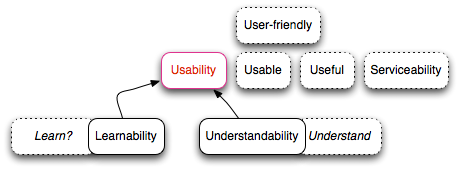
\includegraphics[width=0.4\textwidth]{synonym-graph.pdf}
% \caption{An extensional definition of usability, showing in dashed lines those concepts outside our signifier `bubble'.}
% \label{fig:syngraph}
% \end{figure}

\noindent\textbf{Error analysis} -- We performed error analysis on our results. What we wanted to verify was the percentage of terms retrieved that were unrelated to a signified software quality. For example, we encountered some mail messages from individuals whose email signature included the words ``Usability Engineer''. If the body of the message wasn't obviously about usability, we coded this as a false-positive. Our tests involved randomly selecting messages from the corpora and coding them as relevant or irrelevant. We assessed 100 events per signified term to generate our rates. Table \ref{tbl:error} presents the results of this test. In general, false-positives averaged 23\% of events (i.e., precision was 77\%). \emph{Efficiency} was very high due to the inclusion of the term `ratio' in crash report forms. Recall was 100\%, since the search engine returns all results, but this is a trivial definition, since true recall should be calculated using all events that had that quality as a topic, which we did not assess.

\begin{table}[b]
	\caption{False positive rates}
	\centering
	\label{tbl:error}
\begin{tabular}{|c|c|}
\hline
\rowcolor[gray]{.9} 
Signified quality & F.P. Rate  \\ \hline
Usability & 0.19\\ \hline
Portability & 0.29\\ \hline
Maintainability & 0.13\\ \hline
Reliability & 0.23\\ \hline
Functionality & 0.14 \\ \hline
Efficiency & 0.41\\ \hline
\end{tabular}
\end{table}

\section{Observations and discussion}
\label{sec:observations}
Fig. \ref{fig:naut-usa} plots quality events vs. time for the usability quality in Nautilus. The segmented line connects a number of events for that particular quarter. For example, in the first quarter of 2003, there were approximately 600 (normalized) events in the Nautilus project for usability. The straight line is a linear regression, and the dashed vertical lines represent Gnome project milestones, with which most of the projects we study are synchronized. Fig. \ref{fig:ev-hist} shows the frequency distribution for the same product.

\begin{figure}[h]
\centering
\includegraphics[width=0.45\textwidth]{../data/ev-usab-hist.png}
\caption{Frequency distribution}
\label{fig:ev-hist}
\end{figure}

% \vspace{-2mm}
% \subsection{}
% \vspace{-2mm}
We performed a linear regression of the number of occurrences against the date. The equation of the regression line shows the average value of the number of occurrences as the date increases. A linear relationship may not be a good model of the actual pattern. For example, the number of occurrences may be changing in response to some other variable, such as co-ordinated release dates, or by things such as developer illness. Due to space constraints, Table \ref{tbl:summary} lists only the two longest-lived projects, and $r^2$  -- squared correlation value -- and slope (trend) values for each quality. We ended up with largely conflicting numbers. 

\begin{figure}[b]
\centering
\includegraphics[width=0.45\textwidth]{figures/Nautilus-Usabilityline.png}
\caption{Occurrences per week}
\label{fig:naut-usa}
\end{figure}

\begin{table}
	\caption{Selected summary statistics, normalized}
	\centering
	\label{tbl:summary}
\begin{tabular}{|c|c|c|}
\hline
\rowcolor[gray]{.9} 
Project-Quality &  $r^2$ &  slope \\ \hline
Evolution-Efficiency & 0.07 & -0.38 \\
Evolution-Portability & 0.12 & -0.36 \\
Evolution-Maintainability & 0.05 & -0.27 \\
Evolution-Reliability & 0.08 & -0.29 \\
Evolution-Functionality & 0.05 & 0.92 \\
Evolution-Usability & 0.12 & -1.38 \\
Nautilus-Efficiency & 0.19 & -4.77 \\
Nautilus-Portability & 0.11 & -0.51 \\
Nautilus-Maintainability & 0.37 & -1.49 \\
Nautilus-Reliability & 0.38 & -1.00 \\
Nautilus-Functionality & 0.26 & -4.22 \\
Nautilus-Usability & 0.23 & -7.96 \\
% Totem-Efficiency & 0.03 & -1.86 \\
% Totem-Portability & 0.06 & -0.35 \\
% Totem-Maintainability & 0.00 & 0.02 \\
% Totem-Reliability & 0.02 & 0.19 \\
% Totem-Functionality & 0.16 & -1.87 \\
% Totem-Usability & 0.33 & -1.97 \\
\hline
\end{tabular}
\end{table}

We therefore sought alternative explanations for the patterns seen in our data. We first investigated smaller event windows, based around the period between major Gnome releases; secondly, we used the identified peaks in the data to explore possible causative events. Finally, we examined the role of different qualities in different projects.

\begin{table}
	\caption{Release window technique, normalized}
	\centering
	\label{tbl:windows}
\begin{tabular}{|c|c|c|c|c|}
\hline
\rowcolor[gray]{.9} 
Project-Quality & Release \# & $r^2$ & slope & N\\ \hline
Evolution-Eff. & 2.8 & 0.04 & -0.13 & 20 \\
 & 2.24 & 0.62 & -1.13 & 7\\ \hline
Evolution-Usab. & 2.8 & 0.04 & 1.32 & 24\\
 & 2.24 & 0.04 & -0.52 & 10 \\ \hline
Nautilus-Eff. & 2.8 & 0.00 & -0.23 & 14 \\
 & 2.24 & 0.75 & -6.64 & 4 \\ \hline
Nautilus-Usability & 2.8 & 0.38 & 1.07 & 26\\
 & 2.24 & 0.01 & 0.97 & 14\\
\hline
\end{tabular}
\end{table}

\noindent\textbf{Using release windows} -- It is possible that the peak event occurrences are more strongly correlated with the time period prior to a major release, that is, cyclical. In Fig. \ref{fig:naut-usa}, there seems to be a major upward trend prior to the release of Gnome 2.0, a co-ordinated release. We defined release windows to investigate whether there was higher correlation between number of events and time for selected projects and keywords. Table \ref{tbl:windows} shows our results for selected products and releases (starting with release 2.8, in which Evolution was synchronized with Gnome). For some release dates, we see a high degree of correlation; however, the pattern is not seen in other dates, suggesting the results are not predictive. 

\noindent\textbf{Analysis of key peaks in selected graphs} - The final explanation we explore is that the data are independent of software age, or release cycle, and are instead responding to external events, such as a usability audit. We chose to look at Nautilus, a web browser and file manager, for more detailed analysis. We examined Usability and Portability events, choosing two major peaks to attempt some historical analysis. We first looked at a peak centered around the second quarter of 2002. This coincides with the release of Gnome 2.0 in early June 2002. The mailing list contains a number of comments showing substantial concern over integration with the rest of Gnome 2.0 for theming. Subversion logs and bug comments confirm a connection between the upcoming release and the usability issues. 

We next targeted a peak in the Portability events in the third quarter of 2001. Nautilus 1.0.4 was released early in this period. From exploring the events, there does not seem to be a unifying reason behind this spike. Portability seems to be a quality that is driven by specific bug fixes which need to consider the portability of the final solution. This suggests that not all qualities can be treated the same.

\noindent\textbf{Quality importance and project} -- We hypothesized that certain projects would be more concerned with particular qualities than others. We attempted to characterize the importance of a quality to a project by calculating the mean occurrences of the term over time. We compared the same two projects and terms as above. Table \ref{tbl:quality-project} lists our results. We show the average number of occurrences per week, and then normalize that by dividing by the total number of `events' (eliminating the effect of volume). After considering volume of events, the Nautilus community discusses qualities three times as often as the Evolution community. We intend to do further testing to explore this.

\noindent\textbf{Threats to validity} -- The main threat to construct validity is that our signifiers omit relevant terms or phrases., e.g., ``can't find the submit button" vs. ``usability". Furthermore, we are assuming that projects share the ontology of software quality expressed in the quality model. A more domain-specific taxonomy would be useful. Our data originated from open-source projects, less than ten years old, from the Gnome ecosystem, primarily using \texttt{C} code, so these are threats to external validity.

\begin{table}[b]
	\caption{Quality per project}
	\centering
	\label{tbl:quality-project}
\begin{tabular}{|c|c|c|c|}
\hline
\rowcolor[gray]{.9} 
Quality & Project & Avg. occur. & Norm. occur.\\ \hline
Efficiency & Evolution & 1.51 & \textbf{2.65}\\
 & Nautilus & 1.62 &\textbf{ 6.55}\\\hline
Usability & Evolution & 2.96 & \textbf{5.17}\\
 & Nautilus & 3.52 & \textbf{14.22}\\
\hline
\end{tabular}
\end{table}

\vspace{-2mm}
\section{Conclusions and future work}
\vspace{-2mm}
In the introduction we mentioned our hypothesis that software qualities ought to be of more interest to a community as the project matures. Our data provided no evidence for this hypothesis. We explained a few of the more significant events by examining the possible external causes. These conclusions are necessarily qualitative, but leverage the statistical results for support. We then showed that there seems to be a difference in how different projects treat software qualities.

Our ultimate goal is to be able to extract, from available sources, a list of requirements for a project, so that we can trace not just the `physical' changes in the codebase, but also the evolving features and goals inherent in a project. We plan to continue our experiments with repository mining with this in mind. In all likelihood, we will need to expand both our taxonomy (to be more software development specific) and our data sources (including source code comments or wiki pages, for example).

A secondary direction is related to the social aspect of software development. Each event in our database is initiated by somebody and involves other contributors. It would be interesting to see whether certain individuals are responsible solely for particular software qualities. Hindle et al., in \cite{hindle09icpc}, showed that such information is highly relevant.

% \vspace{-2mm}
% \section{Appendix and acknowledgements}
% \vspace{-2mm}
% \label{appendix}

%Thanks to the comments of the software engineering group at the University of Toronto.
\begin{footnotesize}
\vspace{-2mm}
\bibliography{IEEEabrv,msr}
\vspace{-2mm}
\end{footnotesize}
\end{document}

% I suspect the underlying problem you are having is how
% to cope with requirements churn. From Mary Poppendieck's
% book "Implementing Lean Software Development" there's this
% very valuable tip:
% 
% "If you have requirements churn, you are specifying too
% early".

%Objection: all you've done is take the data and run a simple Grep on it. 
%Well, Abram just used existing ML tools to look at his data


% 
% This paper takes up the question as to whether this can be empirically demonstrated. To test this notion, we begin with a few assumptions. The first is that there is some sort of signal we can capture that will signify that `maintenance' is being done. One approach is to scan code for maintenance activity, using, for example, formal concept analysis~\cite{breu06msr}.